\documentclass[12pt, a4paper]{article}
\usepackage[utf8]{inputenc}
\usepackage[brazilian]{babel} % Hifenização e dicionário
\usepackage[left=3.00cm, right=2.00cm, top=3.00cm, bottom=2.00cm]{geometry}
\usepackage{enumitem} % Para itemsep etc
\usepackage{longtable} % Dependência do longtabu
\usepackage{tabu} % Para melhor criação de tabelas
\usepackage{listings} % Para códigos
\usepackage{lstautogobble} % Códigos indentados corretamente
\usepackage{color} % Para coloração de códigos
\usepackage{zi4} % Para fonte de códigos
\usepackage{parskip} % Linha em branco entre parágrafos em vez de recuo
\usepackage{graphicx}
\usepackage{float}
\usepackage{verbatim}
\usepackage{amsmath}
\usepackage{multirow}
\usepackage[portuguese, ruled, linesnumbered]{algorithm2e}
%\usepackage{algpseudocode}
%\usepackage{algorithm}
\usepackage[autostyle]{csquotes}
\usepackage[breaklinks]{hyperref}

\usepackage{listings}
\lstset{
    autogobble,
    columns=fullflexible,
    showspaces=false,
    keepspaces=true,
    showtabs=true,
    breaklines=true,
    showstringspaces=false,
    breakatwhitespace=true,
    escapeinside={(*@}{@*)},
    commentstyle=\color{greencomments},
    keywordstyle=\color{bluekeywords},
    stringstyle=\color{redstrings},
    numberstyle=\color{graynumbers},
    basicstyle=\ttfamily\footnotesize,
    frame=single,
    framesep=12pt,
    xleftmargin=12pt,
    tabsize=4,
    captionpos=b,
}
\DeclareMathOperator{\argmin}{argmin}
\DeclareMathOperator{\comp}{comp}
\SetKwProg{Fn}{Função}{\string:}{}
\newcommand{\ic}[1]{\textbf{\lstinline{#1}}}

\DeclareGraphicsExtensions{.pdf}

\begin{document}

\begin{center}
    \textsc{Universidade Federal do Rio Grande do Norte} \\
    \textsc{Departamento de Informática e Matemática Aplicada}
\end{center}

\bigskip

\begin{tabular}{@{}ll@{}}
    \emph{Disciplina:} & DIM0406 --- Algoritmos Avançados \\
    \emph{Docente:}    & Sílvia Maria Diniz Monteiro Maia \\
    \emph{Discente:}   & Felipe Cortez de Sá \\
\end{tabular}

\bigskip

\begin{center}
\large \textbf{GRASP-VNS aplicado ao problema de Steiner com rotulação mínima}
\end{center}

\section{Introdução}
Neste relatório são apresentados os algoritmos \emph{Greedy Randomized
Adaptative Search Procedure} e \emph{Variable Neighbourhood Search} para
solução do problema da árvore de Steiner com rotulação mínima. Os princípios de
cada técnica são descritos, assim como a maneira em que foram utilizados para
resolver o problema. É realizada uma análise de complexidade em tempo para as
implementações, identificando os gargalos. Explica-se como foram gerados os
casos de teste e são apresentados resultados comparando o resultado das
execuções para cada técnica, incluindo o algoritmo exato desenvolvido na
segunda unidade. Além disso, é feito um adendo para o relatório do primeiro
trabalho, apresentando os resultados e conclusão previamente faltantes.

\section{Metaheurísticas utilizadas}
As definições seguintes foram adaptadas do \emph{Handbook of Metauheuristics}
\cite{handbook}.

\subsection{GRASP}
O \emph{Greedy Randomized Adaptative Search Procedure} é comumente utilizado em
problemas de otimização combinatória. A cada iteração, é realizada uma fase de
construção, em que se gera uma solução para o problema e posteriormente uma
fase de busca local, procurando um mínimo local na vizinhança da solução
gerada. Se a melhor solução global é encontrada na iteração, atualiza-se a
variável que contém a melhor solução. É um algoritmo de inicialização múltipla,
ou seja, as duas fases são repetidas até o critério de parada ser satisfeito,
podendo esse ser o número de iterações ou o tempo de execução, por exemplo.

Na fase de construção, é criada uma lista de candidatos restritos, possuindo os
elementos que minimizam os custos incrementais. O elemento é selecionado
aleatoriamente dessa lista para entrar na nova solução. O processo é repetido
até obter uma nova solução válida.

\subsection{VNS}
O \emph{Variable Neighbourhood Search} faz uso de múltiplas estruturas de
vizinhança, explorando comumente espaços cada vez mais distantes e maiores,
portanto mais custosos. Para fugir de mínimos locais, o algoritmo possui uma fase
de agitação, em que a solução encontrada pode ser trocada por uma pior a fim de
diversificar a busca, explotando melhor o espaço.

\section{Metaheurística aplicada ao problema}
\subsection{GRASP}
No problema, a fase de construção gera uma lista de candidatos restritos
calculando $ \argmin(\comp(col)) $ para cada cor não utilizada, onde $
\comp(col) $ é o número de componentes conexos do grafo com a coloração $ col $
que incluem pelo menos um nó básico. A operação é repetida até $ \comp(col) $
possuir valor 1, o que significa que foi encontrada uma nova solução válida.

Após a segunda repetição da inicialização múltipla, o primeiro rótulo a ser
adicionado é totalmente aleatório, ou seja, a lista de candidatos é
inicializada como $ {1, 1, ..., 1 } $, explotando melhor o espaço de busca em
vez de escolher sempre rótulos que minimizam $ \comp(col) $.

Após a fase de construção, é feita uma busca local, que consiste em tentar
remover cores da solução e verificar se ainda obtém-se um grafo conexo,
configurando outra solução válida.

%Na implementação, percebeu-se que para grafos com \ic{DENSITY} acima de 50, a
%cardinalidade da coloração atinge o mínimo global identificado pelo algoritmo
%exato nas primeiras iterações. Logo, para deixar o algoritmo mais rápido, o
%critério de parada é a falta de melhoria em três iterações. Para densidades
%menores, a variação entre iterações é maior.

\begin{algorithm}[H]
    \label{alg1}
    \SetAlgoLined
    \DontPrintSemicolon
    %\Entrada{G = (V, E, L)}
    %\Saida{Coloração $ Col $}
    \Fn{\textsc{GRASP}(limite)}{
        $ col^{*} \leftarrow \{\} $ \\
        \Enqto{iterações $ < $ limite}{
            col $ \leftarrow $ \textsc{Construct()} \\
            col $ \leftarrow $ \textsc{Local(col)} \\
            \Se{$ |col| < |col^{*}| $}{
                $ col^* \leftarrow  col $
            }
        }
        \Retorna{col}
    }
    \;
    \Fn{\textsc{Construct}(col)}{
        $ rcl \leftarrow \{\} $ \\
        \Se{iterações $ > $ 2}{
            $ rcl \leftarrow \{1, 1, ..., 1\} $ \\
            col $ \leftarrow $ col $ \cup $ \textsc{Random}(rcl)
        }

        \Enqto{\textsc{Comp}(col) $ > $ 1}{
            $ rcl \leftarrow \argmin \textsc{Comp}(col) $ \\
            col $ \leftarrow $ col $ \cup $ \textsc{Random}(rcl)
        }
        \Retorna{col}
    }
    \;
    \Fn{\textsc{Local}(col)}{
        \Para{cor $ \in $ col}{
            \Se{\textsc{Comp}(col - cor) ==  1}{
                col $ \leftarrow $ col - \{cor\}
            }
        }
        \Retorna{col}
    }
    \caption{\textsc{GRASP}}
\end{algorithm}

\subsection{VNS}
Quando o algoritmo é executado independentemente, a configuração inicial das
cores é totalmente aleatória, isto é, cada elemento do vetor é inicializado
como 0 ou 1 seguindo a distribuição uniforme.

Na fase de agitação, cores de $ col $ são removidas e adicionadas dependendo da
cardinalidade do conjunto. A remoção de cores pode tornar o grafo desconexo,
então é realizado o mesmo procedimento do GRASP para conectar o grafo
escolhendo $ c \in \argmin(\comp(col \cup c)) $ repetidamente.

Em seguida, o mesmo procedimento de busca local utilizado pelo GRASP é
realizado, tentando descartar cores desnecessárias.

\begin{algorithm}[H]
    \caption{\textsc{VNS}}
    \label{alg2}
    \SetAlgoLined
    \DontPrintSemicolon
    \Fn{\textsc{VNS}(limite)}{
        $ col \leftarrow \textsc{GerarVetorAleatório()} $ \\
        \Enqto{iterações $ < $ limite}{
            col $ \leftarrow $ \textsc{Shaking()} \\
            col $ \leftarrow $ \textsc{Local(col)} \\
            k $ \leftarrow $ 1 \\
            \Enqto{$ k < k_{max}$ }{
                \eSe{$ |col^{*}| < |col| $}{
                    $ col^* \leftarrow  col $
                }{
                    ++k
                }
            }
        }
        \Retorna{col}
    }
    \;
    \Fn{\textsc{Shaking}(col)}{
        $ rcl \leftarrow \{\} $ \\
        \Se{iterações $ > $ 2}{
            $ rcl \leftarrow \{1, 1, ..., 1\} $ \\
            col $ \leftarrow $ col $ \cup $ \textsc{Random}(rcl)
        }

        \Enqto{\textsc{Comp}(col) $ > $ 1}{
            $ rcl \leftarrow \argmin \textsc{Comp}(col) $ \\
            col $ \leftarrow $ col $ \cup $ \textsc{Random}(rcl)
        }
        \Retorna{col}
    }
\end{algorithm}

\begin{lstlisting}[caption=Pseudocódigo para VNS, basicstyle=\ttfamily\scriptsize]
vns(col, kmax)
col2 = col
k = 1
while(k <= kmax) {
    shaking(col2, k)
    local(col2)
    if(card(col2) < card(col)) {
        col = col2
        k = 1
    } else {
        ++k
    }
}

shaking(col, k) {
    col2 = col
    for(i in 1..k) {
        if(i <= card(col)) {
            col2[random(cores utilizadas em col)] = 0
        } else {
            col2[random(cores nao utilizadas em col)] = 1
        }
    }

    while(comp(col2) > 1) {
        melhores = argmin comp(c)
        col2[random(melhores)] = 1
    }
}
\end{lstlisting}

\section{Complexidade}
\subsection{GRASP}
\subsection{VNS}

\section{Casos teste utilizados}
Os casos teste utilizados são gerados automaticamente por um programa
\ic{generate.c} de acordo com parâmetros de entrada. Os parâmetros são
\ic{SIZE}, a quantidade de nós do grafo, \ic{COLORS}, o número de rótulos,
\ic{DENSITY}, a proporção de arestas para cada nó, e \ic{BASIC}, a quantidade
de nós básicos. \ic{DENSITY} funciona percorrendo a matriz de adjacência que
representa o grafo e de acordo com a probabilidade definida (sendo 0 e 100
equivalentes a 0\% e 100\%, respectivamente) adicionando ou não uma aresta de
rotulação aleatória ligando dois nós. O arquivo gerado é então passado para o
programa principal.

A fim de comparar os resultados com o trabalho realizado por Cerulli
\cite{cerulli}, os parâmetros dos testes são os mesmos, isto é, tem-se uma
combinação entre \ic{SIZE} $ \in \{50, 100\} $, \ic{COLORS} $ \in \{0.25n,
0.5n, n, 1.25n\} $, \ic{DENSITY} $ \in \{0.2, 0.5, 0.8\}$ e \ic{BASIC} $ \in
\{0.2n, 0.4n\} $. Cada caso teste é executado dez vezes diferentes e são
apresentadas a média, melhor e pior casos e mediana.

O código que gera os arquivos de caso teste para os parâmetros desejados está
em \ic{generate.py}.

\section{Resultados e experimentos comparativos}
\subsection{Comparação com algoritmo exato}
Como pode ser visto nos plots e na tabela, o algoritmo exato funciona bem para
instâncias pequenas do problema, porém os algoritmos metaheurísticos conseguem
lidar com densidades menores e instâncias maiores em menos tempo. Ambas as
metaheurísticas apresentam resultados de mesma qualidade, isto é, mesma
cardinalidade de $ col $ para a maioria das instâncias.

\subsection{Comparação com literatura}
Ao contrário do que se verifica na literatura, a implementação do GRASP
funciona melhor para a maioria dos casos teste, apresentando menos variação
melhor eficiência em tempo.

\section{Conclusões}
Neste trabalho foram feitas as implementações de duas metaheurísticas.
Observou-se que o GRASP obtém soluções melhores e mais consistentes que o VNS,
resultado contrário à literatura. Ambas as metaheurísticas funcionam melhor
para instâncias grandes do problema.

\section{Correções do primeiro trabalho}
\subsection{Técnica utilizada}
O \emph{branch-and-bound} é um algoritmo de otimização que explora o espaço de
busca de maneira mais eficiente que uma enumeração total de soluções possíveis
por força-bruta.  Atualizando o limite inferior continuamente, é possível
eliminar a exploração de regiões não-promissoras do espaço de busca.

\subsection{Resultados}
O tempo de execução para cada instância do caso teste está na tabela 1.
Experimentalmente percebeu-se que se o algoritmo demora mais que cinco
segundos, ele não retornará uma resposta dentro de um minuto. O algoritmo
funciona mais rapidamente para casos em que a densidade é maior. Para \ic{SIZE}
$ = 50 $, costuma falhar na maioria dos casos em que \ic{DENSITY} $ \leq 20 $.
Para tamanhos maiores, falha também quando \ic{DENSITY} $ \leq 50 $.

\subsection{Conclusões}
Neste trabalho verificou-se que o algoritmo exato implementado com
branch-and-bound funciona rapidamente para instâncias pequenas e altas
densidades, mas falha para o restante dos casos.

\subsection{Considerações adicionais}
O código referente ao algoritmo exato foi modificado para aceitar entradas de
um caso de teste, foi comentado mais extensivamente e agora é cronometrado para
possibilitar a análise de resultados.

\section{Tabelas e figuras}

\begin{figure}[H]
    \centering
    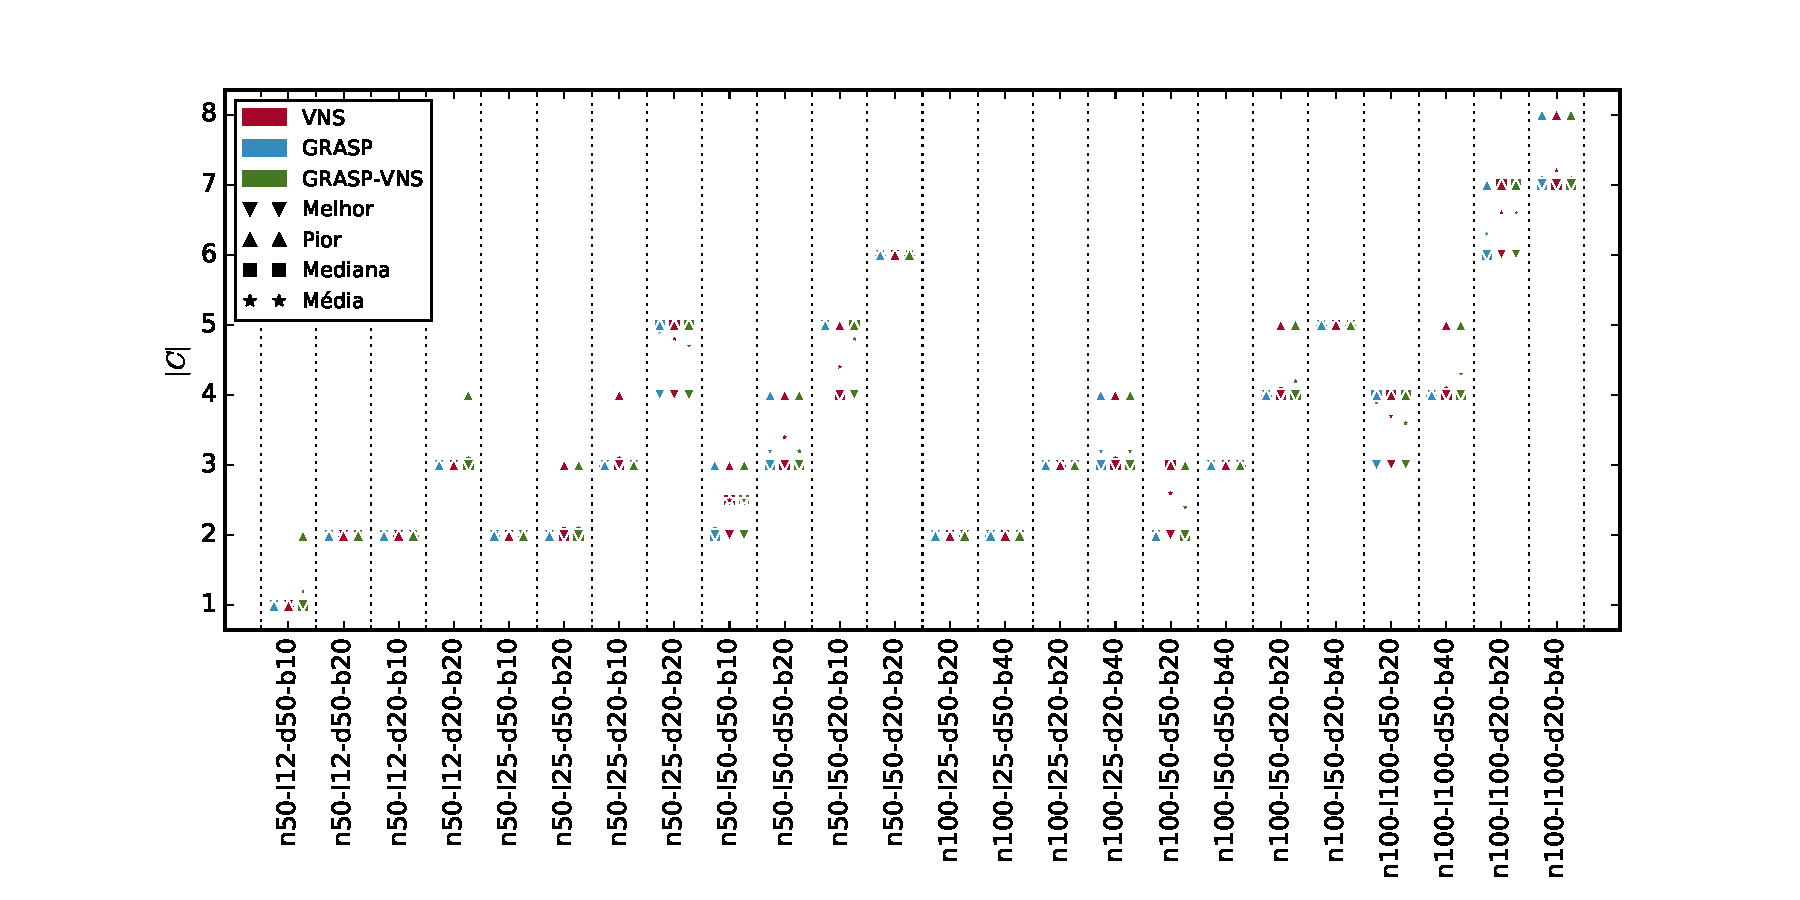
\includegraphics[width=1.00\textwidth]{cardcplot}
    \caption{Plot da qualidade da solução}
    \label{fig:graph_1}
\end{figure}

\begin{figure}[H]
    \centering
    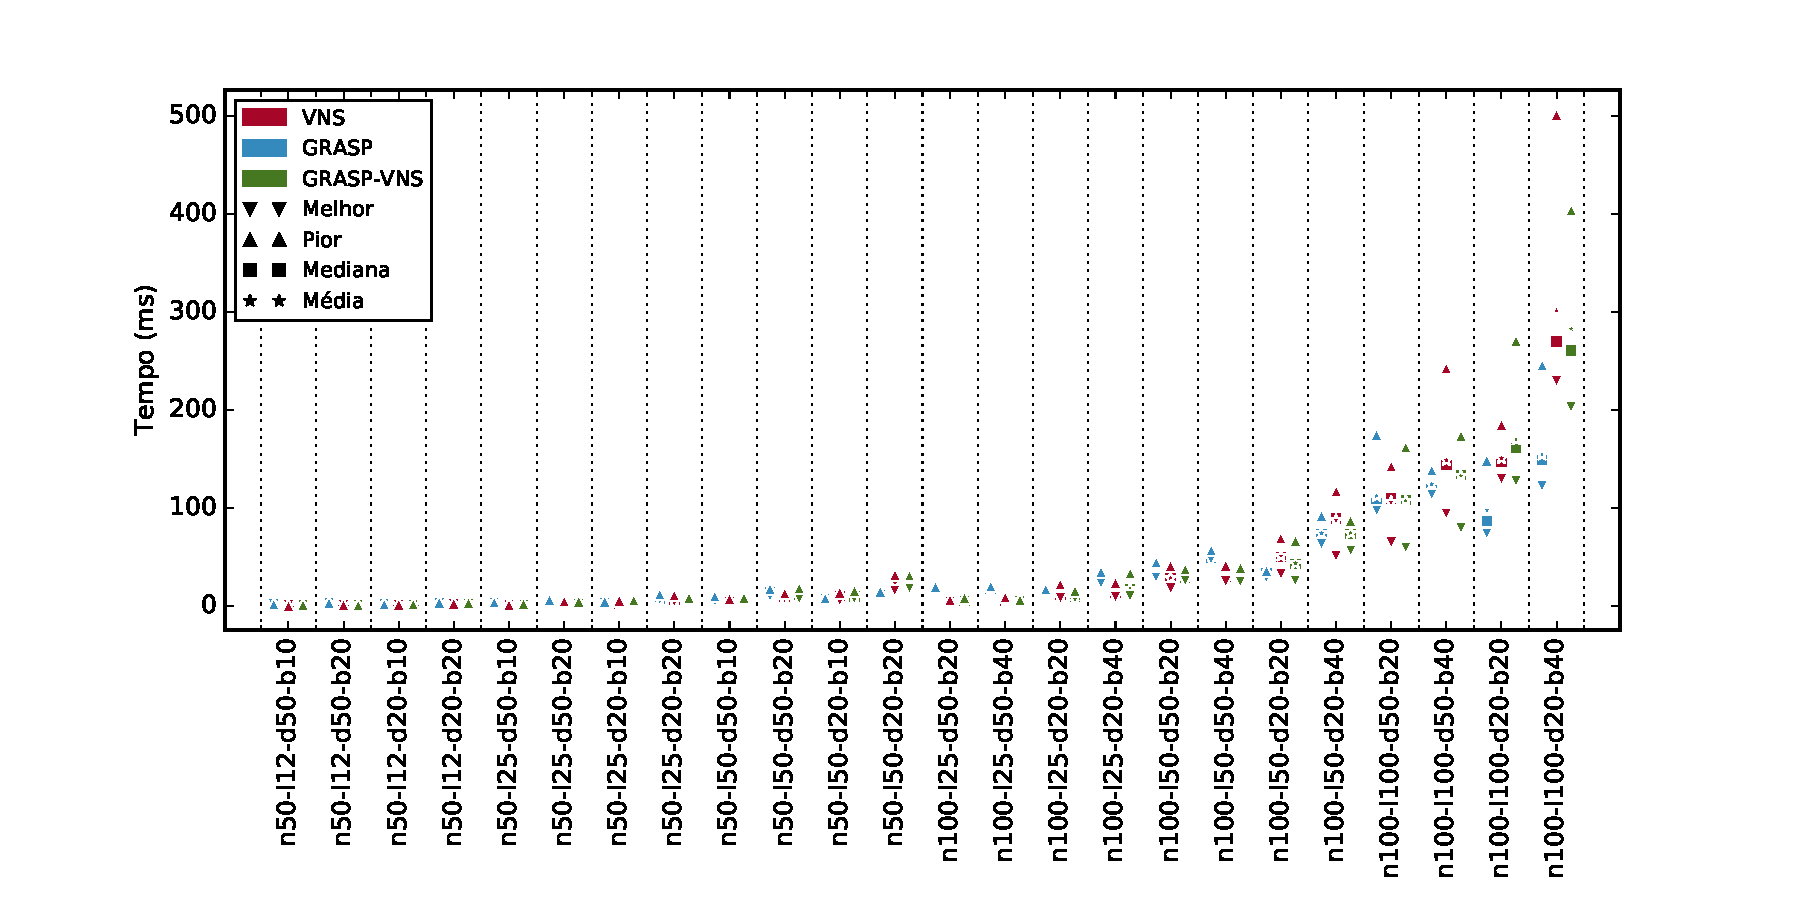
\includegraphics[width=1.00\textwidth]{timeplot}
    \caption{Plot do tempo}
    \label{fig:graph_2}
\end{figure}

%\begin{table}[h]
%\centering
%\tiny
%\begin{tabular}{ |c|c|c|c||c c c| }
\hline
$ n $ & $ l $ & $ d $ & $ b $ & Exato & GRASP & VNS \\
\hline
\multirow{24}{*}{100} & 25 & 80 & 20 &   0.41 &   7.11 &   1.95 \\
& 25 & 80 & 40 &   0.24 &   8.33 &   3.77 \\
\cline{3-4}& 25 & 50 & 20 &   2.81 &  16.70 &   4.97 \\
& 25 & 50 & 40 &   3.31 &  16.20 &   5.28 \\
\cline{3-4}& 25 & 20 & 20 &  36.97 &  13.04 &  16.66 \\
& 25 & 20 & 40 &  82.28 &  21.49 &  17.47 \\
\cline{3-4}\cline{2-2}& 50 & 80 & 20 &   5.60 &  21.73 &   7.52 \\
& 50 & 80 & 40 &   3.87 &  23.37 &  10.47 \\
\cline{3-4}& 50 & 50 & 20 &  17.61 &  29.25 &  19.35 \\
& 50 & 50 & 40 &  57.33 &  37.99 &  28.40 \\
\cline{3-4}& 50 & 20 & 20 &  -1.00 &  36.90 &  46.14 \\
& 50 & 20 & 40 &  -1.00 &  49.40 &  72.14 \\
\cline{3-4}\cline{2-2}& 100 & 80 & 20 & 590.00 &  57.09 &  42.44 \\
& 100 & 80 & 40 & 666.56 &  65.54 &  54.84 \\
\cline{3-4}& 100 & 50 & 20 &  -1.00 &  92.08 &  96.86 \\
& 100 & 50 & 40 &  -1.00 & 121.62 & 148.25 \\
\cline{3-4}& 100 & 20 & 20 &  -1.00 &  65.57 & 155.33 \\
& 100 & 20 & 40 &  -1.00 & 132.17 & 316.71 \\
\cline{3-4}\cline{2-2}& 125 & 80 & 20 & 783.32 &  65.42 &  80.41 \\
& 125 & 80 & 40 & 2071.99 & 109.48 & 112.10 \\
\cline{3-4}& 125 & 50 & 20 &  -1.00 & 110.95 & 146.82 \\
& 125 & 50 & 40 &  -1.00 & 144.25 & 209.87 \\
\cline{3-4}& 125 & 20 & 20 &  -1.00 & 119.30 & 242.61 \\
& 125 & 20 & 40 &  -1.00 & 192.82 & 406.93 \\
\cline{3-4}\cline{2-2}\cline{1-1}\hline
\end{tabular}

%\caption{Tempo (ms)}
%\normalsize
%\end{table}
%
%\begin{table}[h]
%\centering
%\tiny
%\begin{tabular}{ |c|c|c|c||c c c| }
\hline
$ n $ & $ l $ & $ d $ & $ b $ & Exato & GRASP & VNS \\
\hline
\multirow{12}{*}{50} & 12 & 50 & 10 &   1.00 &   1.00 &   1.00 \\
& 12 & 50 & 20 &   2.00 &   2.00 &   2.00 \\
\cline{3-4}& 12 & 20 & 10 &   2.00 &   2.00 &   2.00 \\
& 12 & 20 & 20 &   3.00 &   3.00 &   3.00 \\
\cline{3-4}\cline{2-2}& 25 & 50 & 10 &   2.00 &   2.00 &   2.00 \\
& 25 & 50 & 20 &   2.00 &   2.00 &   2.10 \\
\cline{3-4}& 25 & 20 & 10 &   3.00 &   3.00 &   3.10 \\
& 25 & 20 & 20 &   4.00 &   4.90 &   4.80 \\
\cline{3-4}\cline{2-2}& 50 & 50 & 10 &   2.00 &   2.10 &   2.50 \\
& 50 & 50 & 20 &   3.00 &   3.20 &   3.40 \\
\cline{3-4}& 50 & 20 & 10 &  -1.00 &   5.00 &   4.40 \\
& 50 & 20 & 20 &  -1.00 &   6.00 &   6.00 \\
\cline{3-4}\cline{2-2}\cline{1-1}\multirow{12}{*}{100} & 25 & 50 & 20 &   2.00 &   2.00 &   2.00 \\
& 25 & 50 & 40 &   2.00 &   2.00 &   2.00 \\
\cline{3-4}& 25 & 20 & 20 &   3.00 &   3.00 &   3.00 \\
& 25 & 20 & 40 &   3.00 &   3.20 &   3.10 \\
\cline{3-4}\cline{2-2}& 50 & 50 & 20 &   2.00 &   2.00 &   2.60 \\
& 50 & 50 & 40 &   3.00 &   3.00 &   3.00 \\
\cline{3-4}& 50 & 20 & 20 &  -1.00 &   4.00 &   4.10 \\
& 50 & 20 & 40 &  -1.00 &   5.00 &   5.00 \\
\cline{3-4}\cline{2-2}& 100 & 50 & 20 &  -1.00 &   3.90 &   3.70 \\
& 100 & 50 & 40 &  -1.00 &   4.00 &   4.10 \\
\cline{3-4}& 100 & 20 & 20 &  -1.00 &   6.30 &   6.60 \\
& 100 & 20 & 40 &  -1.00 &   7.10 &   7.20 \\
\cline{3-4}\cline{2-2}\cline{1-1}\hline
\end{tabular}

%\caption{Resultado ($ |C| $)}
%\normalsize
%\end{table}


\begin{thebibliography}{9}

\bibitem{consoli}
S. Consoli, K. Darby-Dowman, N. Mladenovic, J.A. Moreno-Perez.
\textit{Variable neighbourhood search for the minimum labelling Steiner tree
problem}.
Annals of Operations Research, 2009.
\tiny
\\\texttt{\url{https://www.researchgate.net/publication/225327721_Variable_neighbourhood_search_for_the_minimum_labelling_Steiner_tree_problem}}
\normalsize

\bibitem{cerulli}
R. Cerulli, A. Fink, M. Gentili e S. Voß.
\textit{Extensions of the minimum labelling spanning tree problem}.
Journal of Telecommunications and Information Technology, 2006.
\tiny
\\\texttt{\url{https://www.researchgate.net/publication/228668519_Extensions_of_the_minimum_labelling_spanning_tree_problem}}
\normalsize

\bibitem{handbook}
Glover, F., Kochenberger, G. A. et al.
\textit{Handbook of Metaheuristics}.
Kluwer Academic Publishers

\end{thebibliography}

\end{document}
